\documentclass{beamer}
\usepackage{ctex, hyperref}
\usepackage[T1]{fontenc}
\usepackage{latexsym,amsmath,xcolor,multicol,booktabs,calligra}
\usepackage{graphicx,pstricks,listings,stackengine}
\def\cmd#1{\texttt{\color{red}\footnotesize $\backslash$#1}}
\def\env#1{\texttt{\color{blue}\footnotesize #1}}
\definecolor{deepblue}{rgb}{0,0,0.5}
\definecolor{deepred}{rgb}{0.6,0,0}
\definecolor{deepgreen}{rgb}{0,0.5,0}
\definecolor{halfgray}{gray}{0.55}
\lstset{
	basicstyle=\ttfamily\small,
	keywordstyle=\bfseries\color{deepblue},
	emphstyle=\ttfamily\color{deepred},
	stringstyle=\color{deepgreen},
	numbers=left,
	numberstyle=\small\color{halfgray},
	rulesepcolor=\color{red!20!green!20!blue!20},
	frame=shadowbox,
}

%---------------------------------------------------

\author{HocRiser}
\title{数论初步}
\institute{吉林大学 20级唐计}
\date{2021年1月27日}
\usepackage{waseda}

\begin{document}

\kaishu
\begin{frame}
	\titlepage
	\begin{figure}[htpb]
		\begin{center}
			\includegraphics[width=0.2\linewidth]{pic/HocRiser.jpg}
		\end{center}
	\end{figure}
\end{frame}

\begin{frame}
	\tableofcontents[sectionstyle=show,subsectionstyle=show/shaded/hide,subsubsectionstyle=show/shaded/hide]
\end{frame}

%---------------------------------------------------

\section{概述}

\subsection{符号与约定}

\begin{frame}
\begin{itemize}[<+-| alert@+>]
	\item $a \in \mathbb{R}$,$b \in \mathbb{Z}$,$b \leq a$,$b+1>a$,则称$b = \lfloor a \rfloor$
	\item $a,b \in \mathbb{Z}$,定义$a \bmod b=a-\lfloor\frac{a}{b}\rfloor*b$
	\item $a,b \in \mathbb{N*}$,若$b \bmod a = 0$,则称$a$整除$b$,记为$a|b$,并称$a$为$b$的约数,$b$为$a$的倍数。
	\item $a,b \in \mathbb{N*}$,最大的$n(n \in \mathbb{N*})$使得$n|a$,$n|b$,则称$n$为$a$与$b$的最大公约数,记为$n = gcd(a,b)$
	\item $a,b \in \mathbb{N*}$,最小的$n(n \in \mathbb{N*})$使得$a|n$,$b|n$,则称$n$为$a$与$b$的最小公倍数,记为$n = lcm(a,b)$
	\item $a,b \in \mathbb{N*}$,若$gcd(a,b)=1$,则称$a,b$互素,记为$a \perp b$
\end{itemize}
\end{frame}

\subsection{同余与模运算}

\begin{frame}
\begin{itemize}[<+-| alert@+>]
	\item 设$a,b \in \mathbb{Z}$,若$a \bmod c = b\bmod c$,则称$a$与$b$同余,记为$a \equiv b\pmod c$
	\item 自然数域下的模运算的性质有:
	\begin{itemize}[<+-| alert@+>]
		\item $(a \bmod c) + (b \bmod c) \bmod c= (a+b)\bmod c$
		\item $(a \bmod c)(b \bmod c)\bmod c = (ab)\bmod c$
		\item $(a\bmod c)^b \bmod c=a^b \bmod c$
	\end{itemize}
\end{itemize}
\end{frame}

\begin{frame}
\begin{itemize}[<+-| alert@+>]
	\item 由此,我们可以得到同余的性质。设$c \in \mathbb{N*}$,$n \in \mathbb{Z}$:
	\item 若$a \equiv b\pmod c$,则$a-b\equiv 0\pmod c$
	\item 若$a \equiv b\pmod c$,则$a+n \equiv b+n\pmod c$
	\item 若$a \equiv b\pmod c$,则$a-n \equiv b-n\pmod c$
	\item 若$a \equiv b\pmod c$,则$a\times n \equiv b\times n\pmod c$
	\item 若$a \equiv b\pmod c$,则$a^n \equiv b^n\pmod c$($n \in \mathbb{N*}$)
	\item $a+nc \equiv a\pmod c$
\end{itemize}
\end{frame}

\begin{frame}
\begin{itemize}[<+-| alert@+>]
	\item 同时我们可以定义模意义下的运算。
	\item 对于模m意义下的运算,任意$n \in \mathbb{N}$,可以找到$n' \in [0,m)$使得$n \equiv n' \pmod m$。
	\item 传统的加法、减法、乘法,仍然具有封闭性,结合律,分配律,“1元素”,“0元素”等性质。
	\item 若$ac=bc$,则当$gcd(c,m)=1$时,$a=b$
\end{itemize}
\end{frame}

\begin{frame}
\begin{itemize}[<+-| alert@+>]
	\item 对于$n \in \mathbb{N*}$,一个整数集中的数模n所得的余数域,称为剩余系。
	\item 设$m \in \mathbb{N*}$,若$r_0,r_1,\cdots,r_{m-1}$为$m$个整数,并且两两模m不同余,则$r_0,r_1,\cdots,r_{m-1}$叫作模$m$的一个完全剩余系。
	\item 设$m \in \mathbb{N*}$,以$C_r(r=0,1,\cdots,m-1)$表示所有形如$km+r(k\in \mathbb{Z}$的整数组成的集合,则$C_0,C_1,\cdots,C_{m-1}$称为$m$的剩余类。
	\item $m$个剩余类每个取一个代表元,即为完全剩余系。
	\item 与$m$互素的各个等价类中取一个代表元,称为缩系。$\varphi(m)$表示这样的数的个数,称为$Euler$函数。
\end{itemize}
\end{frame}

\subsection{素数}

\begin{frame}
\begin{itemize}[<+-| alert@+>]
	\item 当一个数$n(n \in \mathbb{Z}且n > 1)$的约数只有$2$个($1$和他本身)时,称之为素数/质数。 当一个数的约数大于$2$个时,称之为合数。
	\item $Euler$函数$\varphi(n)$基本性质:
		\begin{itemize}[<+-| alert@+>]
			\item $\varphi(n)=n\prod(1-\frac{1}{p_i})$
			\item 若$m\perp n$,则$\varphi(mn)=\varphi(m)\varphi(n)$
			\item 若$p|n$,则$\varphi(pn)=p\varphi(n)$
			\item 若$p \in \mathbb{P}$,则$\varphi(p)=p-1$
		\end{itemize}
\end{itemize}
\end{frame}

\section{数论定理}

\subsection{算术基本定理}

\begin{frame}
\begin{itemize}[<+-| alert@+>]
	\item 算术基本定理(唯一分解定理):
		\begin{itemize}[<+-| alert@+>]
			\item 任意大于$1$的自然数都可以唯一地写为若干素数的积的形式(从小到大)
		\end{itemize}
	\includegraphics[width=0.8\linewidth]{pic/divisor.jpg}
\end{itemize}
\end{frame}

\subsection{费马小定理、欧拉定理与威尔逊定理}

\begin{frame}
\begin{itemize}[<+-| alert@+>]
	\item 费马小定理:
		\begin{itemize}[<+-| alert@+>]
			\item $p \in \mathbb{P}$,$a \in \mathbb{N*}$,$p \nmid a$,则$a^{p-1} \equiv 1 \pmod p$
		\end{itemize}
	\item 欧拉定理:
		\begin{itemize}[<+-| alert@+>]
			\item $p,a \in \mathbb{N*}$,$p \perp a$,则$a^{\varphi(p)} \equiv 1 \pmod p$
		\end{itemize}
	\item 威尔逊定理:
		\begin{itemize}[<+-| alert@+>]
			\item $p \in \mathbb{P}$等价于$(p-1)! \equiv -1 \pmod p$,否则余数为$0$,$p=4$时例外。
		\end{itemize}
\end{itemize}
\end{frame}

\subsection{中国剩余定理}

\begin{frame}
\begin{itemize}[<+-| alert@+>]
	\item 对于线性同余方程组$x \equiv a_i \pmod {m_i}$且$m_i$两两互质,无论$a_i$取值如何一定有解。
	\item $x \equiv \sum a_{i}m_{i}m_{i}^{-1} \pmod M(M=\prod m_i)$
	\item 扩展中国剩余定理:\url{https://blog.csdn.net/clove_unique/article/details/54571216}
\end{itemize}
\end{frame}

\section{数论算法}

\subsection{辗转相减与辗转相除}
\begin{frame}
\begin{itemize}[<+-| alert@+>]
	\item 设$a>b$,$令d=gcd(a,b)$,则$d|a$,$d|b$,故$d|a-b$
	\item 由此得到辗转相减法:每次将大的数减去小的数,直到一个数为$0$,此时另一个数即为$gcd$
	\item 令$d=gcd(a,b)$,则$d|(a\bmod b)$
	\item 由此得到辗转相除法:每次将大的数对小的数取模,直到一个数为$0$,此时另一个数即为$gcd$
	\item 每次大的数至少缩小一半,故复杂度为$\log(\max(a,b))$
\end{itemize}
\end{frame}

\subsection{扩展欧几里得算法}
\begin{frame}
\begin{itemize}[<+-| alert@+>]
	\item 裴蜀定理:$a,b \in \mathbb{Z}$,存在无穷多组整数对$(x,y)$满足不定方程$ax+by=d$,其中$d=gcd(a,b)$
	\item 在求$gcd(a,b)$的同时,可以求出上述方程的一组整数解。
	\item 递归计算:假设已经求出$(b \bmod a,a)$的一组解$(x_0,y_0)$,满足$(b \bmod a)x_0+ay_0=d$
	\item 可以得到$(b-a\lfloor\frac{b}{a}\rfloor)x_0+ay_0=d$
	\item 整理得到$a(y_0-\lfloor\frac{b}{a}\rfloor x_0)+bx_0=d$
\end{itemize}
\end{frame}

\subsection{BSGS算法}

\begin{frame}
\includegraphics[width=1.2\linewidth]{pic/BSGS1.png}
\end{frame}

\begin{frame}
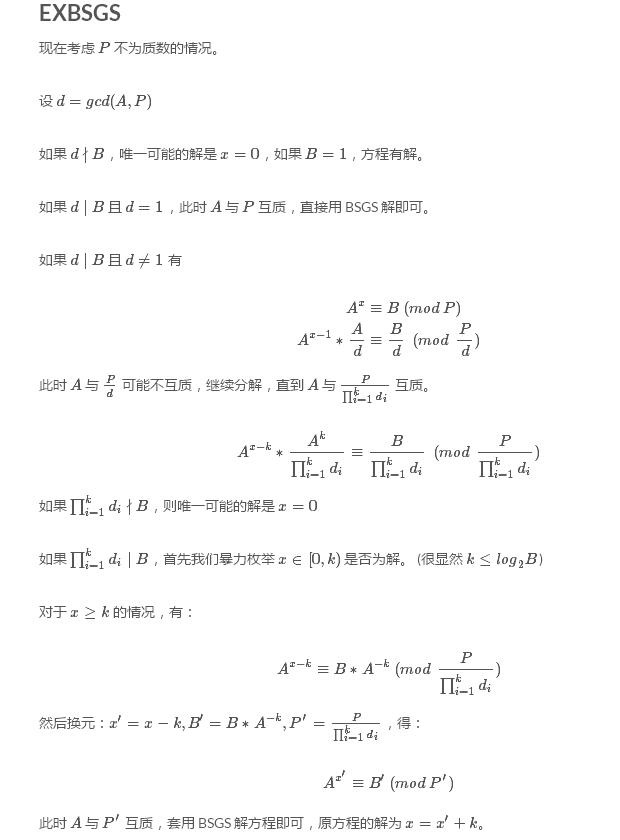
\includegraphics[width=1.0\linewidth]{pic/BSGS2.png}
\end{frame}

\begin{frame}
\includegraphics[width=0.8\linewidth]{pic/BSGS3.jpeg}
\end{frame}

\begin{frame}
\includegraphics[width=0.8\linewidth]{pic/BSGS4.jpeg}
\end{frame}

\subsection{Eratosthenes筛法与线性筛法}

\begin{frame}
\begin{itemize}[<+-| alert@+>]
	\item 朴素素数判定:$\forall n \notin \mathbb{P}$,$\exists y \in (1,\sqrt{n}]$,使得$y|n$
	\item 朴素筛法:从$2$到$n$,枚举每个数的倍数(除去自身)并标记为合数
	\begin{itemize}[<+-| alert@+>]
		\item 时间复杂度:$O(n+\frac{n}{2}+\cdots+\frac{n}{n})~O(n \ln n)$
	\end{itemize}
	\item Eratosthenes筛法:从$2$到$n$,枚举每个\textbf{素}数的倍数(除去自身)并标记为合数
	\begin{itemize}[<+-| alert@+>]
		\item 时间复杂度:$O(n \ln n \ln n)$
	\end{itemize}
	\item Euler筛法:对于每个素数$p$,从小到大枚举它的所有倍数$i*p(i>1)$并标记为合数,直到$p|i$
	\begin{itemize}[<+-| alert@+>]
		\item 每一个数只会被它最小的质因子筛到一次
		\item 时间复杂度:$O(n)$
	\end{itemize}
\end{itemize}
\end{frame}

\subsection{递推求逆元}

\begin{frame}
\begin{itemize}[<+-| alert@+>]
	\item 若$ab \equiv 1 \pmod p$,则称$b$为$a$在$\bmod p$意义下的乘法逆元,记为$a^{-1} \equiv b \pmod p$
	\item $\frac{a}{b}=a \times b^{-1} \pmod p$
	\item 由欧拉定理:$a^{\varphi(p)} \equiv a^{-1} \pmod p(a\perp p)$
	\item 不互素时考虑用exgcd解不定方程
\end{itemize}
\end{frame}

%---------------------------------------------------

\end{document}